\documentclass{simple}

\title[De ce securitate?]{De ce să învăț securitate?}
\institute{Talks by Softbinator (\#149)}
\author[Răzvan Deaconescu]{Răzvan Deaconescu \\
razvan.deaconescu@upb.ro}
\date{13 mai 2021}

\begin{document}

\frame{\titlepage}

\begin{frame}{}
  \centering
  \LARGE
  wargame
\end{frame}

\begin{frame}{WarGames (film, 1983)}
  \begin{figure}
    \centering
    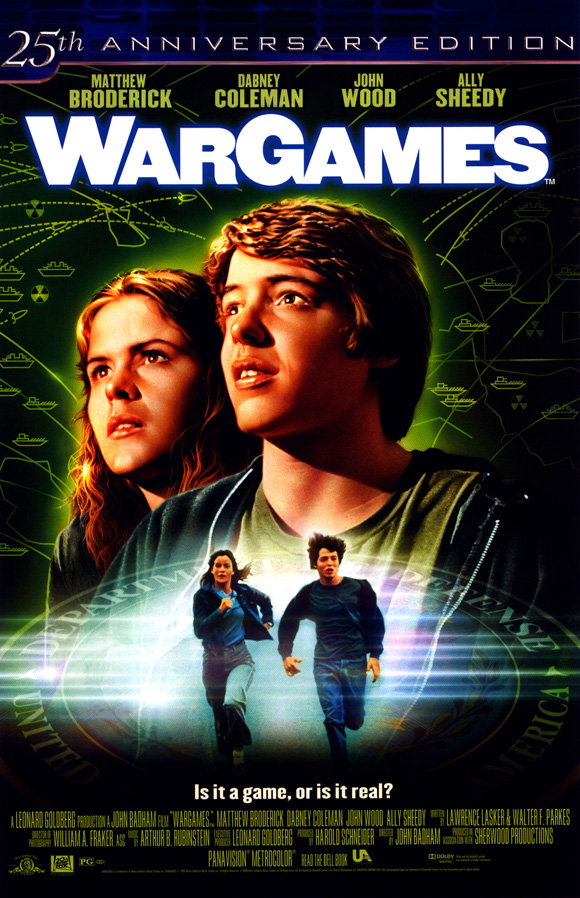
\includegraphics[width=0.4\textwidth]{img/wargames-film.jpg} \\
    \tiny{\url{https://moviejunkyard.wordpress.com/2013/05/22/wargames1983/}}
  \end{figure}
\end{frame}

\begin{frame}{Cyber Wargame}
  \begin{figure}
    \centering
    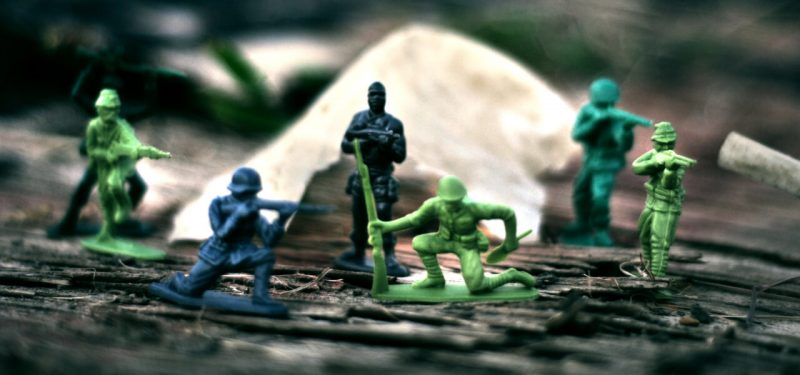
\includegraphics[width=\textwidth]{img/cyber-wargame.jpg} \\
    \tiny{\url{https://techbeacon.com/security/how-train-your-next-security-crisis-let-wargames-begin}}
  \end{figure}
\end{frame}

\begin{frame}{Wargames}
  \begin{itemize}
    \item \url{https://overthewire.org/wargames/}
    \item \url{https://io.netgarage.org/}
    \item \url{https://www.wechall.net/}
    \item \url{https://w3challs.com/}
    \item \url{http://pwnable.kr/}
  \end{itemize}
\end{frame}

\begin{frame}{Wargames}
  \centering
  \pause
  \vspace{0.5cm}
  \Large{securitate} \\
  \pause
  \vspace{0.5cm}
  \Large{scenariu / setup} \\
  \pause
  \vspace{0.5cm}
  \Large{\textbf{challenge}} \\
  \pause
  \vspace{0.5cm}
  \Large{fun}
\end{frame}

\begin{frame}{Challenge / Provocare}
  \centering
  \pause
  \vspace{0.5cm}
  \Large{ne-trivial} \\
  \pause
  \vspace{0.5cm}
  \Large{ceva nou} \\
  \pause
  \vspace{0.5cm}
  \Large{exciting} \\
  \pause
  \vspace{0.5cm}
  \Large{catharsis} \\
  \pause
  \vspace{0.5cm}
  \Large{improvement}
\end{frame}

\begin{frame}{Scrisul de cod - challenge?}
  \centering
  \pause
  \vspace{0.5cm}
  \Large{trivial?} \\
  \pause
  \vspace{0.5cm}
  \Large{same old?} \\
  \pause
  \vspace{0.5cm}
  \Large{boring?} \\
  \pause
  \vspace{0.5cm}
  \Large{next?}
\end{frame}

\begin{frame}{Nu e vorba de scrisul de cod}
  \centering
  \pause
  \textit{First, solve the problem. Then, write the code.} \\
  \vspace{3mm}
  \hfill \textit{John Johnson} \\
\end{frame}

\begin{frame}{Securitate / Wargames vs. Dezvoltare / scris cod vs. Bug hunting}
  \centering
  \pause
  \vspace{0.5cm}
  \Large{trivial vs. provocator} \\
  \pause
  \vspace{0.5cm}
  \Large{comun vs. nou} \\
  \pause
  \vspace{0.5cm}
  \Large{tern vs. exciting} \\
  \pause
  \vspace{0.5cm}
  \Large{thrill of the hunt + catharsis vs. checklist} \\
  \pause
  \vspace{0.5cm}
  \Large{îmbunătățire vs. platitudine} \\
  \pause
  \vspace{0.5cm}
  \Large{It's more about the journey than the destination.}
\end{frame}

\begin{frame}{De ce să învăț securitate?}
  \centering
  \pause
  \vspace{0.5cm}
  \Large{provocare} \\
\end{frame}

\begin{frame}{}
  \centering
  \LARGE
  CTF (Capture the Flag)
\end{frame}

\begin{frame}{Capture the Flag (video game)}
  \begin{figure}[!htbp]
    \centering
    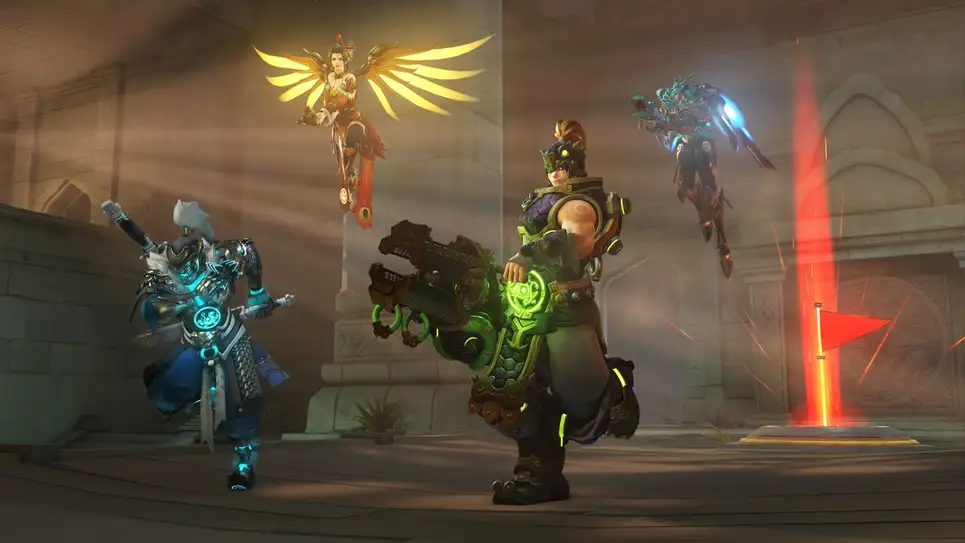
\includegraphics[width=\textwidth]{img/overwatch-ctf.png} \\
    \tiny{\url{https://kotaku.com/overwatchs-new-ctf-map-is-a-big-improvement-1822886612}}
  \end{figure}
\end{frame}

\begin{frame}{Capture the Flag (security)}
  \begin{figure}
    \centering
    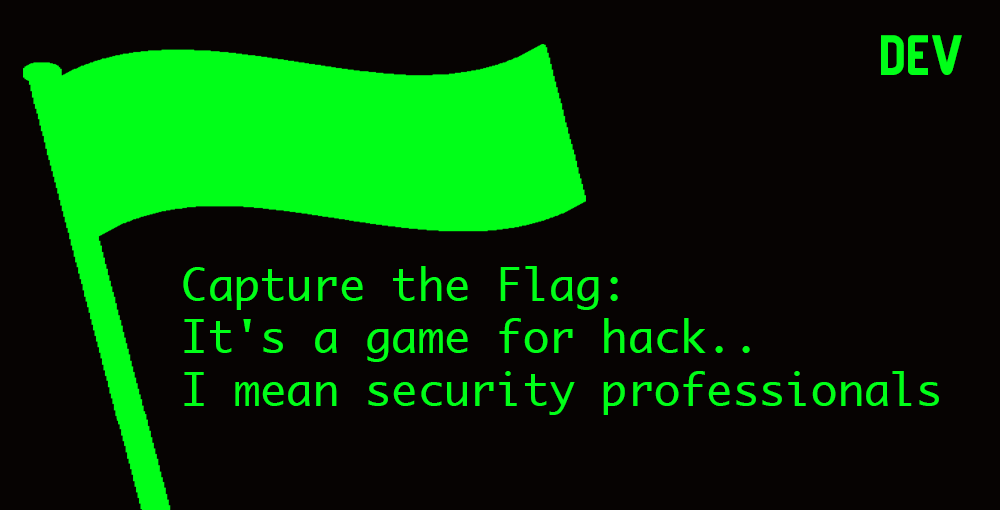
\includegraphics[width=\textwidth]{img/security-ctf.png} \\
    \tiny{\url{https://ro.pinterest.com/pin/465489311475951778/}}
  \end{figure}
\end{frame}

\begin{frame}{CTF}
  \begin{itemize}
    \item \url{https://ctftime.org/}
    \item \url{https://picoctf.org/}
    \item \url{https://capturetheflag.withgoogle.com/}
    \item \url{https://dctf.def.camp/}
    \item \url{https://unbreakable.ro/}
  \end{itemize}
\end{frame}

\begin{frame}{CTF}
  \centering
  \pause
  \vspace{0.5cm}
  \Large{time-bound} \\
  \pause
  \vspace{0.5cm}
  \Large{diversitate de scenarii} \\
  \pause
  \vspace{0.5cm}
  \Large{echipă}
\end{frame}

\begin{frame}{Sarcini în echipă}
  \centering
  \pause
  \textit{9 women cannot make a baby in one month.} \\
  \vspace{3mm}
  \hfill \textit{Fred Brooks} \\
\end{frame}

\begin{frame}{CTF Team Work}
  \centering
  \pause
  \vspace{0.5cm}
  \Large{distribuție de sarcini} \\
  \pause
  \vspace{0.5cm}
  \Large{rotație de sarcini} \\
  \pause
  \vspace{0.5cm}
  \Large{utilitare colaborative} \\
  \pause
  \vspace{0.5cm}
  \Large{sinergie co-echipieri} \\
  \pause
  \vspace{0.5cm}
  \Large{planificare} \\
  \pause
  \vspace{0.5cm}
  \Large{pregătire anterioară} \\
  \pause
  \vspace{0.5cm}
  \Large{formare și menținere echipă}
\end{frame}

\begin{frame}{CTF Community}
  \centering
  \pause
  \vspace{0.5cm}
  \Large{write ups} \\
  \pause
  \vspace{0.5cm}
  \Large{mentorat} \\
  \pause
  \vspace{0.5cm}
  \Large{organizat competiții}
\end{frame}

\begin{frame}{De ce să învăț securitate?}
  \centering
  \vspace{0.5cm}
  \Large{provocare} \\
  \pause
  \vspace{0.5cm}
  \Large{echipă, comunitate} \\
\end{frame}

\begin{frame}{Ce trebuie pentru securitate?}
  \begin{itemize}
    \pause
    \item rețelistică
    \pause
    \item sisteme de operare
    \pause
    \item software engineering
    \pause
    \item hardware
    \pause
    \item compilatoare
    \pause
    \item matematică
    \pause
    \item utilitare de dezvoltare, colaborare
    \pause
    \item linie de comandă
  \end{itemize}
\end{frame}

\begin{frame}{Ce (mai) trebuie pentru securitate?}
  \begin{itemize}
    \pause
    \item răbdare
    \pause
    \item perseverență
    \pause
    \item răbdare
    \pause
    \item perseverență
    \pause
    \item răbdare
    \pause
    \item perseverență
    \pause
    \item să te înțelegi bine cu ceilalți
  \end{itemize}
\end{frame}

\begin{frame}{Pentru securitate \ldots}
  \centering
  \pause
  \vspace{0.5cm}
  \Large{\ldots{} trebuie multe, dar \ldots} \\
  \pause
  \vspace{0.5cm}
  \Large{\ldots{} le înveți, având ca \textbf{obiectiv} securitatea.}
\end{frame}

\begin{frame}{}
  \centering
  \pause
  \vspace{0.5cm}
  \Large{It's more about the journey than the destination, but \ldots} \\
  \pause
  \vspace{0.5cm}
  \Large{\ldots{} you have to have a destination.} \\
  \pause
  \vspace{0.5cm}
  \Large{Security is the destination. The goal. OS, networking, compilers are the journey.}
\end{frame}

\begin{frame}{}
  \begin{figure}[!htbp]
    \centering
    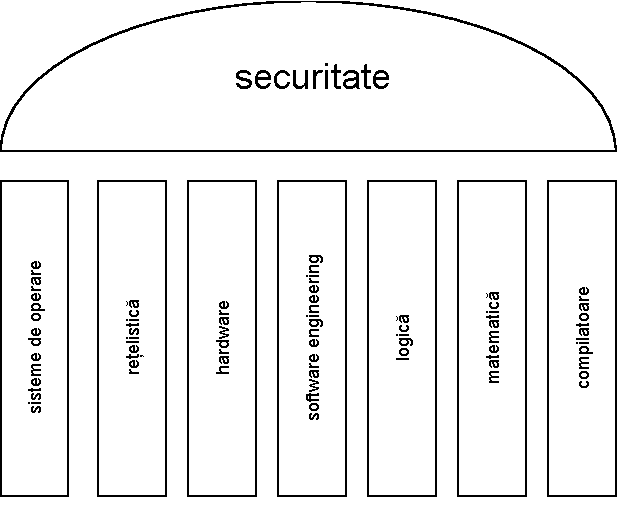
\includegraphics[width=0.8\textwidth]{img/security-deps.pdf}
  \end{figure}
\end{frame}

\begin{frame}{De ce să învăț securitate?}
  \centering
  \vspace{0.5cm}
  \Large{provocare} \\
  \vspace{0.5cm}
  \Large{echipă, comunitate} \\
  \pause
  \vspace{0.5cm}
  \Large{înveți celelalte lucruri}
\end{frame}

\begin{frame}{Nu e greu pentru începători?}
  \centering
  \pause
  \vspace{0.3cm}
  \large{Dimpotrivă.} \\
  \pause
  \vspace{0.3cm}
  \large{Cea mai des întâlnită întrebare la începători: Ce să învăț? De unde încep?} \\
  \pause
  \vspace{0.3cm}
  \large{Cel mai greu pentru începător e să aibă întrebări. Probleme. Țeluri.} \\
  \pause
  \vspace{0.3cm}
  \large{Computers are useless. They can only give you answers.} \\
  \vspace{2mm}
  \hfill \textit{Pablo Picasso} \\
  \pause
  \vspace{0.3cm}
  \large{(Comunitatea de) securitate(a) îți dă probleme. Scenarii. Wargames. CTF.} \\
  \pause
  \vspace{0.3cm}
  \large{Ce mai aștepți?}
\end{frame}

\begin{frame}{De ce să învăț securitate?}
  \centering
  \vspace{0.5cm}
  \Large{provocare} \\
  \vspace{0.5cm}
  \Large{echipă, comunitate} \\
  \vspace{0.5cm}
  \Large{înveți celelalte lucruri} \\
  \pause
  \vspace{0.5cm}
  \Large{îți dă cadrul de învățăre: probleme, provocări, scenarii}
\end{frame}

\begin{frame}{De unde încep?}
  \begin{itemize}
    \item picoCTF: \url{https://picoctf.org/}
    \item OverTheWire: \url{https://overthewire.org/wargames/}
    \item Security Summer School: \url{https://security.cs.pub.ro/summer-school/wiki/}
  \end{itemize}
\end{frame}

\begin{frame}{}
  \centering
  \LARGE
  Have fun and happy hacking, cracking, breaking, smashing, \textbf{learning}!
\end{frame}

\begin{frame}{Resurse}
  \begin{itemize}
    \item slide-urile prezentării: \url{https://www.slideshare.net/razvandeaconescu/}
    \item cod sursă prezentare: \url{https://github.com/razvand/slides}
    \item Security Summer School: \url{https://security.cs.pub.ro/summer-school/wiki/}
    \item resurse agregate de wargames / CTF: \url{https://zaratec.github.io/ctf-practice/}
    \item alte resurse agregate de wargames / CTF: \url{https://fareedfauzi.gitbook.io/practice-ctf-list/}
  \end{itemize}
\end{frame}

\end{document}
